\lecture{2010-01-26}

\subsection{Potenzreihen -- Differentialgleichungen}

\begin{description}
\item[Airy-DGL]
\begin{equation*}
	\ddot{u}(t) - t \cdot u(t) = 0
\end{equation*}
(1880 -- Radio/Lichtwellen)\\der Koeffizient $t$ ist hier variabel, der Ansatz über $\euler^{\lambda t}$ deshalb nicht zulässig

\item[Schwingungsgleichung]
\begin{equation*}
	\ddot{u} + u = 0
\end{equation*}
hier ist der Koeffizient konstant, der Ansatz $u(t) = \euler^{\lambda t}$ funktioniert deshalb

\end{description}
obige Gleichungen sind beide lineare Differentialgleichungen 2. Ordnung

\subsubsection*{Entwicklungssatz}
gegeben: DGL 2. Ordnung, linear
\begin{equation*}
	\ddot{u}(t) + a(t)\dot{u}(t) + b(t)u(t) = s(t)
\end{equation*}
%
$s(t)$ wird als Quellterm, Source, Inhomogenität oder auch Anregung bezeichnet.
\begin{equation*}
	\text{Theorie: }Ax = b
\end{equation*}

\begin{theorem}[Entwicklungssatz]
	Alle Koeffizienten $a(t)$, $b(t)$ und Anregung $s(t)$ sind als Potenzreihen darstellbar $\implies u(t)$ ist als Potenzreihe darstellbar (Analog-Rechner).
\end{theorem}

\begin{example}[zur Schwingungsgleichung: $\ddot{u} + u = 0$]
Gesucht wird:
\begin{equation*}
	u(t) = \sum \limits_{k = 0}^\infty c_k t^k
\end{equation*}
\paragraph{Idee}Koeffizientenvergleich, dazu Potenzreihe einsetzen in die DGL:
\begin{align*}
	\dot{u}(t) &= \sum \limits_{k = 1}^\infty k c_k t^{k - 1} = \sum \limits_{k = 0}^\infty (k + 1) c_{k + 1} t^k \\
	\ddot{u}(t) &= \sum \limits_{k = 2}^\infty k (k - 1) c_k t^{k - 2} = \sum \limits_{k = 0}^\infty (k + 2)(k + 1) c_{k + 2} t^k
\end{align*}
Nach Einsetzen ergibt sich
\begin{align*}
	\sum \limits_{k = 0}^\infty (k + 2)(k + 1) c_{k + 2} t^k + \sum \limits_{k = 0}^\infty c_k t^k &= 0
	\intertext{Abgleich zu $t^k$ (mit $k \geq 0$):}
	(k + 1)(k + 2)c_{k + 2} + c_k &= 0
\end{align*}
Damit gilt:
\begin{equation*}
	\left.
	\begin{aligned}
		c_2, c_4, \ldots \text{ sind Funktionen von }c_0 &= u(0) \\
		c_3, c_5, \ldots \text{ sind Funktionen von }c_1 &= \dot{u}(0) \\
	\end{aligned}
	\right\}\text{Anfangswerte (werden vorgegeben)}
\end{equation*}

\paragraph{Auflösung}
\begin{align*}
	k &= 2m && c_{2m + 2} = \frac{-1}{(2m + 1)(2m + 2)}\underbrace{c_{2m}}_{\text{Cosinus-Anteil}} \\
	k &= 2m + 1 && c_{2m + 1} = \frac{-1}{(2m + 2)(2m + 3)}\underbrace{c_{2m - 1}}_{\text{Sinus-Anteil}}
\end{align*}
Aus dem $\euler^{\lambda t}$-Ansatz folgt:
\begin{equation*}
	\left.
	\begin{aligned}
		\text{$\lambda$ ist imaginär } u(t) = \alpha_1 \cos(t) + \alpha_2 \sin(t) \\
		\text{$\alpha_1$, $\alpha_2$ aus Anfangswerten}
	\end{aligned}
	\right\}\text{Passt exzellent zusammen!}
\end{equation*}

\end{example}

\begin{example}[Airy-DGL]
\begin{equation*}
	\ddot{u}(t) - t \cdot u(t) = 0
\end{equation*}
Variabler Koeffizient $t$
\begin{align*}
	\underbrace{\sum \limits_{k = 0}^\infty (k + 1)(k + 2) c_{k + 2}}_{\ddot{u}(t)} t^k - \underbrace{t \underbrace{\sum \limits_{k = 0}^\infty c_k t^k}_{u(t)}}_{\sum \limits_{k = 0}^\infty c_k t^{k + 1} = \sum \limits_{k = 1}^\infty c_{k - 1} t^k} &= 0 \\
	\sum \limits_{k = 1}^\infty \bigl(\underbrace{(k + 1)(k + 2)c_{k + 2} - c_{k - 1}}_{= 0}\bigr) t^k + 2\underbrace{c_2}_{= 0} &= 0
	\intertext{($c_0$ und $c_1$ aus Anfangswerten)}
\end{align*}

\end{example}

\section{Integration}

\subsection{Bestimmtes Integral}
\label{sub:bestInt}

\begin{center}
	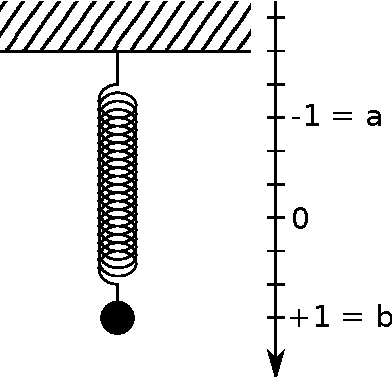
\includegraphics[width=0.4\textwidth]{include/20100126-1.pdf}
\end{center}

\begin{example}
	gesucht: Die Arbeit $W$, um eine Feder ein Stück zu dehnen
	\begin{align*}
		F & \text{: konstant} \\
		s & \text{: Wegstück, um das die Feder gedehnt wird} \\
		\text{Arbeit} &= \text{Kraft} \cdot \text{Weg}
	\end{align*}
	Feder aus Position $a$ nach Position $b$ gezogen. Kraft zur Federdehnung sei ortsabhängig.
\end{example}

\noindent Diagramm:
\begin{center}
	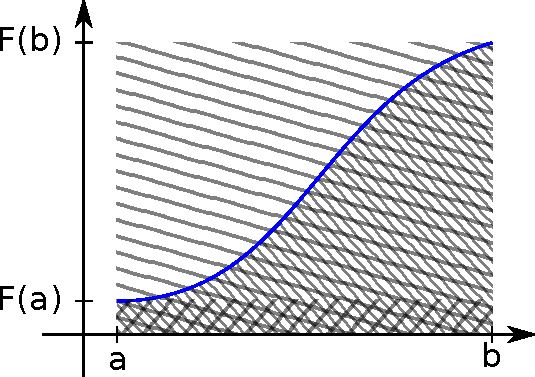
\includegraphics[width=0.4\textwidth]{include/20100126-2.pdf}
\end{center}
Kraftverlauf $F(x)$, Arbeit $W$: eingeschlossene Fläche

\begin{equation*}
	\text{Einschachteln von $W$:}\left.
	\begin{aligned}
		\text{unten: } & F(a) (b - a) \\
		\text{oben: } & F(b) (b - a) \\
	\end{aligned}
	\right\}
	\begin{aligned}
		& F(a) (b - a) \leq W \leq F(b) (b - a) \\
		& \text{technische Frage: Flächenberechnung} \\
	\end{aligned}
\end{equation*}

\paragraph{Historie} $F_\square = a^2$, $F_{\text{Rechteck}} = ab$, $F_\bigcirc = r^2\pi$

\paragraph{Arbeitsprogramm} Flächenberechnung -- Riemann-Integral

\begin{description}
  \item[1. Idee] untere/obere Grenzen aus Rechteckkonstruktion

\begin{enumerate}
	\item 2 Rechtecke gefunden, die den Wert von $W$ grob abschätzen
	\item Bekannt: $F_{\text{Rechteck}} = ab$
	\item Bekannt: Kraftverlauf $F(x)$
\end{enumerate}

  \item[2. Idee] Unterteile $[a, b]$ in Teilintervalle
\begin{center}
	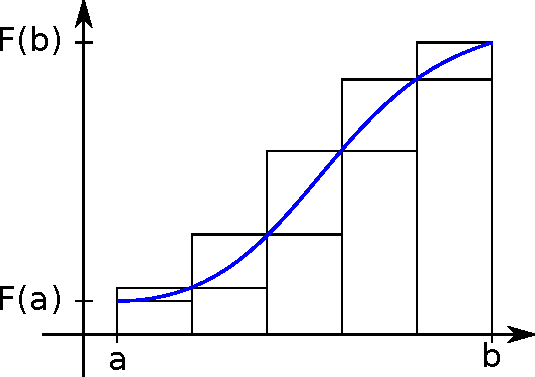
\includegraphics[width=0.4\textwidth]{include/20100126-3.pdf}
\end{center}
einbeschriebene Rechtecke $\leq$ Fläche \\
umgeschriebene Rechtecke $\geq$ Fläche

\end{description}